\chapter{Casos de Uso}
\label{chapter:casos_de_uso}

% Escrever sobre caso de uso do sistemas
No capítulo \ref{chapter:projeto} descrevemos o funcionamento da Interface e sua comunicação com a linguagem MQTT. Este capítulo busca demonstrar o funcionamento do sistema em hardwares com a interface implementada pelos softwares descritos na seção \ref{section:codigos_fonte} disponível no Apêndice. São aplicações simples que mostram a facilidade e a escalabilidade do sistema, além de demonstrar como o sistema pode ser implementado em plataformas.

\section{Medição de temperaturas de CPU}
\label{section:temp_cpu}

\textbf{obs:} \textit{Para reproduzir este teste, é necessário seguir as instruções encontradas no Apêndice}.

Este exemplo tem como objetivo medir a temperatura da CPU de um console com baseado em suas atividades, serviços e processos em execução. A aplicação pode ser escalada para a obtenção de outras informações da CPU e do sistema, podendo assim disponibilizar análises de desempenho da plataforma, além de montar perfis de uso do sistema e administrar seu uso.

A escalabilidade do sistema será testada em partes, a primeira será analisar medições de temperatura de uma CPU de um console. Em seguida comparar medições de temperatura da CPU com um ESP32 e por último analisar temperatura de múltiplas CPUs.

Para isso precisaremos utilizar uma instância da classe Publisher disponível  \ref{subsection:publishers_javascript} como e no console a ter informações de temperatura a ser coletadas e uma instãncia do Subscriber \ref{subsection:subscribers_javascript} para receber estas temperaturas via MQTT e persisti-las em banco de dados. Ambas as aplicações utilizarão as APIs em Javascript, utilizando Node.js para coletar as informações do sistema, implementar o Publisher, o Subscriber, o driver para MongoDB (também disponível em anexo) e a geração de um gráfico utilizando a plataforma plotly \cite{plotly}. Isso foi implementado no código \ref{subsection:teste_fonte}.

CPUs são tecnologias feitas por transistores. Milhões de aglomerações de MOSFETS que começam a  ter perda de perfomance no processador conforme o aumento de temperatura, em \cite{jose}, pode-se observar os efeitos do aumento de  temperatura nos parâmetros do MOSFET especialmente na queda de mobilidade e na velocidade de saturação que provocam perda de perfomance. CPUs modernas são capazes de ajustar suas frequências operacionais, a fim de reduzir seu consumo de energia ou fornecer a máxima potência, conforme necessário e possuem também  proteção térmica extremamente robusta. Se a unidade começar a operar acima do limite térmico, ela começará a reduzir a frequência para evitar uma falha catastrófica.

\begin{figure}[h!]
\centering
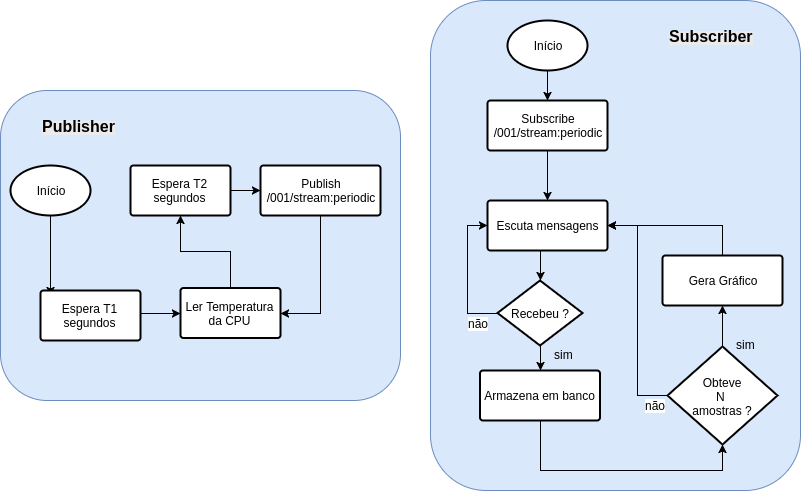
\includegraphics[width=11.5cm]{./02_Capitulos/02_Cap4/figures/fluxo_controle_temp}
\caption{Diagrama de fluxos do Publisher e do Subscriber}
\label{fig:4.1.0/fluxo_controle_temp}
\end{figure}

% Falar sobre o diagrama de fluxo
A \ref{fig:4.1.0/fluxo_controle_temp} mostra todo o fluxo das duas aplicações, o Publisher publica em no tópico \textit{/001/stream:periodic}, a informação coletada a cada T1=3 segundos e espera T2=1 antes de enviar. O Subscriber escuta este tópico e persiste ao chegar uma mensagem de dados pelo Data Stream, ao atingir N=100 amostras, um gráfico de Temperatura da CPU principal pela Data-Hora de inserção é gerado com as últimas 100 inserções no banco.


% Inserção no banco
Repare que a medição depende da data e da hora de inserção no banco, o tempo de chegada até a persistência varia muito com a latência e com o processamento da aplicação, desta forma temos uma medida mais constante. A \ref{fig:4.1.0/compass} mostra o formato de dado armazenado, com a ferramenta Compass para visualização de dados do MongoDB. Repare que lidamos com a estrutura de dados em documento porém obrigatoriamente todo documento da Interface possui o timestamp da inserção no banco, o campo data é o objeto de dados em medição. A comunicação com o banco pode ser feita por uma instância da classe MongoDataClient em   \ref{subsection:subscribers_javascript} que cuida da inserção com  o \textit{timestamp} e o objeto de dados em \textit{data}.

\begin{figure}[h!]
\centering
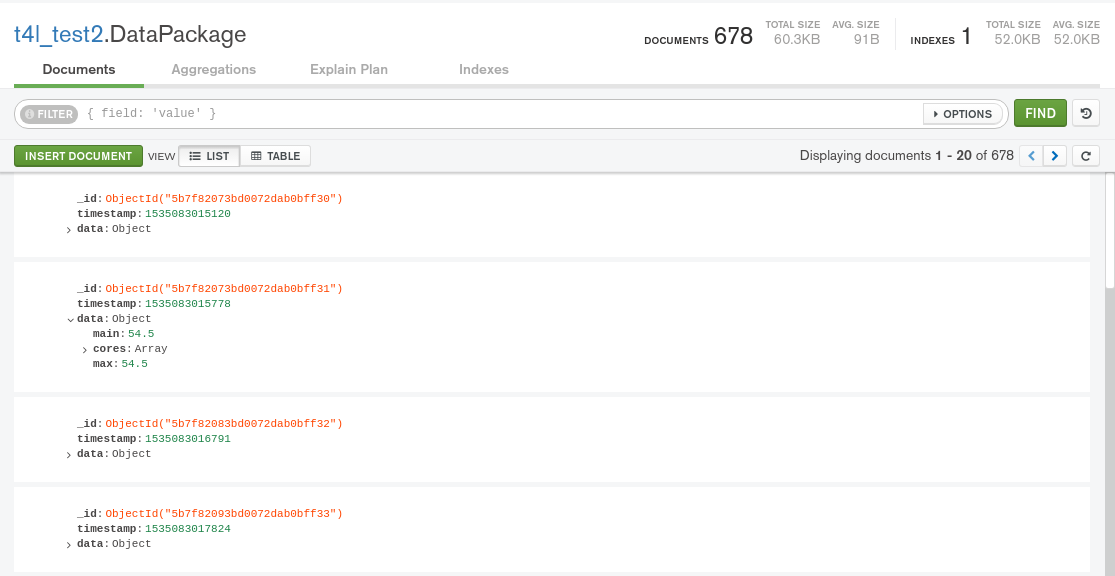
\includegraphics[width=15cm]{./02_Capitulos/02_Cap4/figures/compass}
\caption{Visualização dos dados armazenados em documento em uma coleção do MongoDB}
\label{fig:4.1.0/compass}
\end{figure}

% Visualização com o plotly
A visualização de dados é feita pela ferramenta Plotly, um serviço que fornece uma interface para criar, editar e analisar gráficos, basta criar uma conta, gratuíta ou paga, e o usuário poderá criar gráficos na plataforma web ou através de APIs implementadas em múltiplas linguagens de programação conhecidas. A aplicação do Subscriber utiliza da segunda opção com o módulo plotly.js, a implementação em Javascript da plataforma. A cada N=100 amostras são produzidos gráficos como o da  \ref{fig:4.1.0/cpu-temp_1}.


\begin{figure}[h!]
\centering
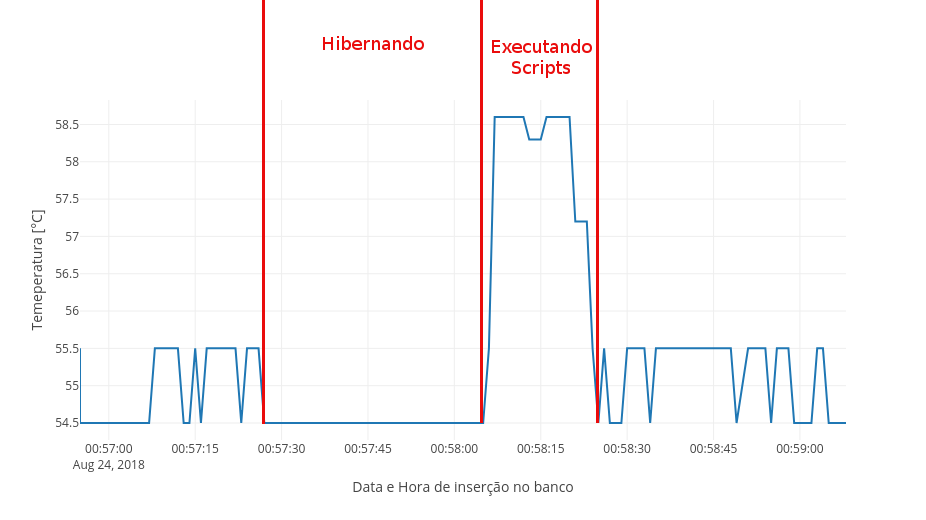
\includegraphics[width=16cm]{./02_Capitulos/02_Cap4/figures/cpu-temp_1}
\caption{Comportamento da temperatura em três momentos}
\label{fig:4.1.0/cpu-temp_1}
\end{figure}

A \ref{fig:4.1.0/cpu-temp_1} mostra a variação da temperatura de uma CPU da Intel Core I7 em três momentos. O gráfico começa no primero momento onde só os processos básicos do computador estão em execução, mantendo a temperatura constante, logo em seguida entra o momento onde o computador está hibernando o que leva a uma pequena baixa na temperatura. O terceiro momento descreve o comportamento quando o computador executa o MATLAB em um script que exige capacidade de processamento, causando uma leve alta de temperatura, mas não tão lata devido a capacidade do processador e depois estabilizando e voltando ao primeiro momento. Com isso fechando o ciclo das aplicações.


Finalizada a medição de uma CPU, pode-se escalar para uma Análise mais elaborada, junto as medições desta CPU core i7, foi acrescentada uma aplicação contendo um Publisher em um ESP32. Conforme descrito no capítulo anterior na \ref{fig:3.3.4/esp32-arch}, o ESP32 é um MCU que possui módulos WiFi e sensor de temperatura interno, facilitando a medição, como trata-se de um Microcontrolador foi utilizado a implentação em C++ \ref{subsection:teste-plataformas}, uma implementação síncrona.


\begin{figure}[h!]
\centering
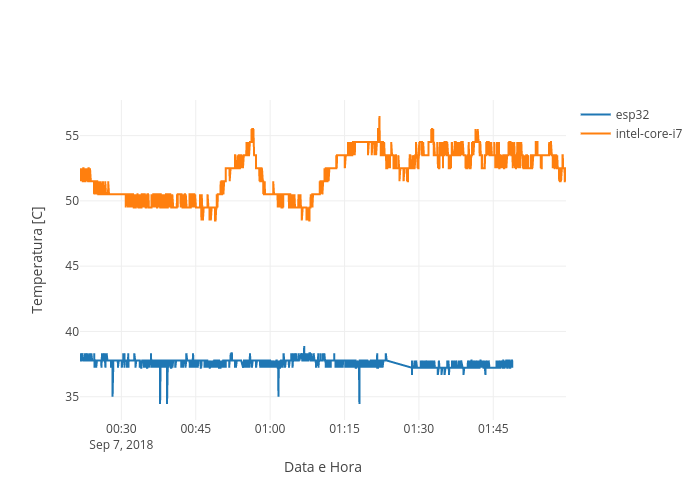
\includegraphics[width=16cm]{./02_Capitulos/02_Cap4/figures/temp-device-3}
\caption{Comparação das temperaturas com uma CPU core i7 e ESP32}
\label{fig:temp-devices-3}
\end{figure}

Ambas as plataformas foram configuradas para enviar informações de temperatura com intervalos de um segundo, durante um período de cerca de uma hora e meia, ao completar 10 mil amostras totais, um gráfico é gerado. Cada plataforma contribui com cerca de metade das amostras, porém cada uma possui uma rotina e capacidade de processamento, fora o tempo de envio para Broker, é de se esperar que o número de amostras de cada um não seja igual.
Pela \ref{fig:temp-devices-3} pode-se observar as diferenças de temperatura e o comportamento das duas CPUS. O ESP32 com sua arquitetura mais simples, mantem-se relativamente constante a 30 graus Celsius,  isso pode ser explicado devido ao fato do ESP estar rodando somente um programa devido suas limitações.
A CPU i7 varia sua temperatura em torno de 50 graus Celsius, possuindo variações mais bruscas, devido ao fato do processador está executando múltiplo processos. Durante este experimento o computado da CPU foi usado normalmente, passando por cenários de hibernação até o uso do Browser, recebendo requisições de páginas da web, assistindo vídeos e áudios, provocando as variações de temperatura semelhantes ao primeiro teste.


Por último o sistema foi utilizado em um teste em múltiplos computadores com processadores distintos no Laboratório PROSAICO. A finalidade foi observar o comportamento e a robustês da aplicação ao receber dados de múltiplas fontes em larga escala (cerca de 15 mil amostras totais no banco).

\begin{figure}[h!]
\centering
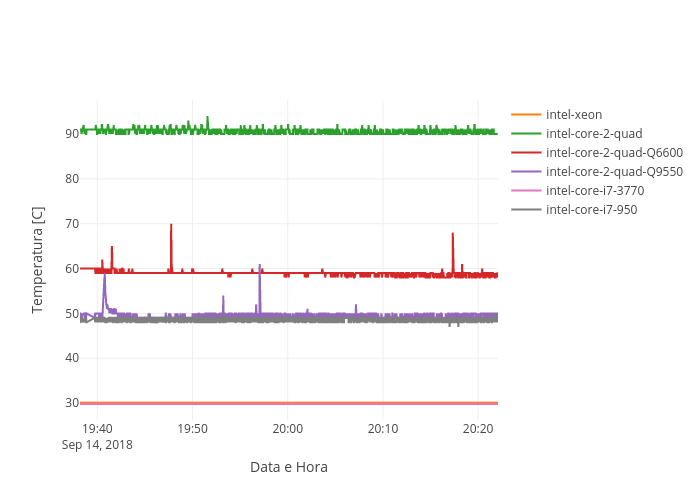
\includegraphics[width=16cm]{./02_Capitulos/02_Cap4/figures/temp-devices-5}
\caption{Comparação das temperaturas em múltiplos processandores}
\label{fig:temp-devices-5}
\end{figure}

Na \ref{fig:temp-devices-5}, observa-se vários níveis de temperatura média entre os processadores, todos executando processos comuns dos sistemas operacionais em máquinas Windows e Linux. Esta diferença está atrelada aos fatores de resfriagem térmica e a capacidade de processamento. Vale ressaltar alguns comportamentos. Os dois processadores de temperatura mais baixa, por volta de 30 graus Celsius possuem gabinetes mais novos e apresentam um sistema de resfriamento melhor que os mais antigos. Já o processador que registrou uma maior temperatura média, fora o processador do computador usado como servidor Web e IoT do laboratório, hospedando o Broker Mosquitto do sistema, inclusive. Dois fatores contribuiram para essa mudança abrupta de tecnologia, os processos executados dos serviços, porém majoritariamente pela manutenção do resfriamento do processador, foi detectado que a CPU estava sem pasta térmica, grande responsável pela troca de calor na própria.


%\section{Aplicação: Automação Residencial}
%\label{section:residencial}
%
%Para validar o baixo custo do sistema, as próximas seções tem o foco em simular o orçamento de dois projetos. Um feito para a indústria e outro em redes domésticas para automações residenciais. Serão propostos cenários de aplicações reais, capazes de confirmar a premissa do projeto.
%Como vimos no capítulo de projetos, o sistema pode ser instalado em plataformas mais sofisticadas, contendo sistemas operacionais e hardware dedicado. Mas nestes cenários utilizaremos o hardware mínimo que é compatível com o sistema e atua satisfatoriamente na aplicação.
%
%
%O caso em estudo é a automação parcial de uma residência. Como pode ser visto em  \ref{fig:5.1.0/planta-casa}, a casa possui dois quartos, sala de estar, dois banheiros, cozinha, área de serviço e varanda. O objetivo é monitorar a temperatura local, o consumo de energia, detectar aberturas de portas e janelas de entrada da residência para fins de segurança e acionamento de luzes.
%
%Para isso é necessário acionadores para a sala e cozinha, mais os quartos, totalizando cerca de 4 pontos de luz para acionar, o mesmo vale para os sensores de temperatura, no qual farão a média de temperatura da casa. Para controle de consumo de energia, nos limitaremos as tomadas de eletrodomésticos e eletrônicos, que representam a maior parte do consumo, para um ponto na sala, nos quartos, na tomada da geladeira, micro-ondas e lavadora, cerca de 6 tomadas a colocar sensores de tensão e corrente AC para cálculo da potência. Serão colocados sensores magnéticos para detectar abertura de portas e janelas, na porta de entrada, na porta da varanda, nas janelas do quarto e na área de serviço.
%
%\begin{figure}[h!]
%\centering
%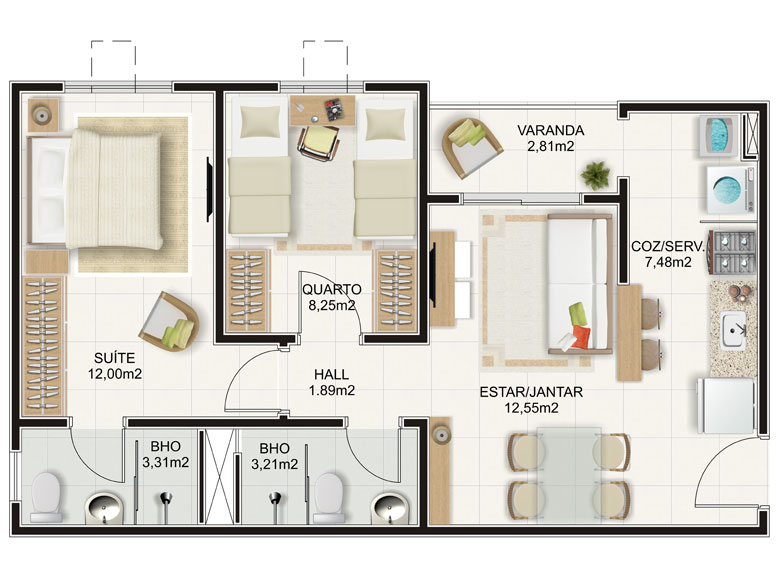
\includegraphics[width=13cm]{./02_Capitulos/02_Cap5/figures/planta-casa}
%\caption{Planta baixa de residência de dois quartos, retirado de \cite{decorandocasas}}
%\label{fig:5.1.0/planta-casa}
%\end{figure}
%
%Nota-se pela \ref{table:planta-casa}, com menos de R\$ 2000,00 pode-se instalar um sistema robusto para automatizar uma casa. O projeto já conta que a residência possui uma rede WiFi e se a casa tiver um PC, pode-se abater do custo do servidor.
%
%
%\begin{table}[h!]
%\centering
%\caption{Orçamento de um sistema simples para automação da residência da \ref{fig:5.1.0/planta-casa}}
%\begin{tabular}{|l|l|l|l|l|}
%\hline
%Item                & Descrição                    & Qtde & Unidade (R\$) & Total (R\$) \\ \hline
%esp32               & Módulo de aquisição          & 4    & \$30.00       & \$120.00    \\ \hline
%DHT11               & Sensor de temperatura        & 4    & \$10.00       & \$40.00     \\ \hline
%P8                  & Módulo sensor de tensão      & 6    & \$20.00       & \$120.00    \\ \hline
%Acs712 - 5a         & Módulo sensor de corrente    & 6    & \$15.00       & \$90.00     \\ \hline
%Ssr-25              & Relé Estado Sólido           & 4    & \$30.00       & \$120.00    \\ \hline
%Desktop             & Servidor Local               & 1    & \$600.00      & \$600.00    \\ \hline
%Sensores Magnéticos & Sensores de abertura         & 6    & \$40.00       & \$240.00    \\ \hline
%Infraestrura        & Caixas de proteção, fios etc & 1    & \$500.00      & \$500.00    \\ \hline
%\multicolumn{4}{|l|}{TOTAL:}                                              & \$1,830.00  \\ \hline
%\end{tabular}
%\label{table:planta-casa}
%\end{table}
%
%
%\section{Aplicação: Controle de Iluminação de Postos de combustível}
%\label{section:posto}
%
%
%Essa é uma aplicação que pode ser usado no comércio assim como na indústria. Trata-se de uma central que controla via rede local as iluminações de postos de combustível. Estes possuem uma fonte de luz bastante potente na testeira(Parte de cima do posto) e no Totem (presente na entrada do posto, onde são mostrados os preços dos combustíveis). A infraestrutura do projeto não é complexa, Necessitará de um módulo ESP32 para processamento e envio dos acionamentos, relés de estado sólido, disjuntores de curva C, uma bateria que converte CA em CC, geralmente baterias similares as de celulares satisfazem, isso para o interfaciamento entre a rede elétrica e o sistema digital de controle. Por fim tudo isso ficará presente em uma caixa com vedação perto da caixa de energia do posto.
%
%Para montar a rede Wifi local, será utilizado um roteador dedicado, configurando uma rede local, não é necessário a conexão a internet neste ponto do projeto. O ESP32 irá se conectar a rede por wps \cite{linksys}, O broker irá ser instalado em um desktop na parte administrativa do posto. O diferencial da aplicação está na aplicação. O frentista responsável poderá acessar a rede e um servidor HTTP irá fornecer uma página web no qual ele pode enviar comandos de acionamento das luzes e até agendar o acionamento destas para um horário específico.
%
%
%\begin{table}[h]
%\caption{Infraestrura para sistema de controle de iluminação de  postos de Combustíveis}
%\begin{tabular}{|l|l|l|l|l|}
%\hline
%Item           & Descrição                   & Qtde & Unidade (R\$) & Total (R\$) \\ \hline
%esp32          & Módulo de aquisição         & 1    & \$30.00       & \$30.00     \\ \hline
%Disjuntor      & Curva C                     & 4    & \$40.00       & \$160.00    \\ \hline
%P8             & Módulo sensor de tensão     & 6    & \$20.00       & \$120.00    \\ \hline
%Acs712 - 5a    & Módulo sensor de corrente   & 6    & \$15.00       & \$90.00     \\ \hline
%Ssr-25         & Relé Estado Sólido          & 4    & \$30.00       & \$120.00    \\ \hline
%Desktop        & Servidor Local              & 1    & \$600.00      & \$600.00    \\ \hline
%TP-Link AC1350 & Roteador Wireless           & 1    & \$280.00      & \$280.00    \\ \hline
%Infraestrura   & Caixa de proteção, fios etc & 1    & \$700.00      & \$700.00    \\ \hline
%\multicolumn{4}{|l|}{TOTAL}                                         & \$2,100.00  \\ \hline
%\end{tabular}
%\label{table:posto}
%\end{table}		
%
%Na \ref{table:posto}, como temos um sistema trifásico é necessário mais acionadores, como  as ferramentas utilizadas para o projeto da aplicação são de escopo aberto e gratuitas, não possuímos despesas neste aspecto. Deve-se planejar um local para que a caixa de controle consiga captar um sinal estável do roteador, e é recomendável configura-lo para enviar dados em um canal menos congestionado. O sensores de tensão e corrente foram adicionados caso seja adicionado ao projeto um monitoramento de consumo de energia.